\chapter{Результаты исследования}

На рисунке \ref{img:1} представлено распределение нормализованных оценок пользователей.

\begin{figure}
	\begin{center}
		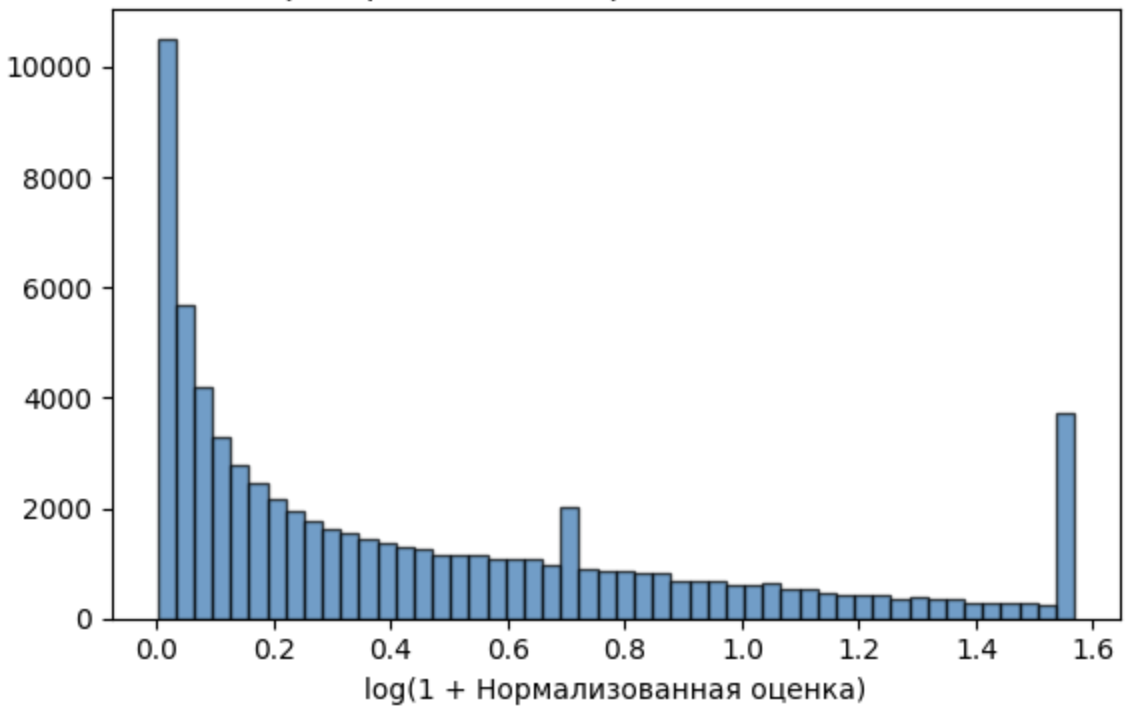
\includegraphics[width=\textwidth]{images/1.png}
	\end{center}
	\caption{Распределение нормализованных оценок пользователей}
	\label{img:1}
\end{figure}

\begin{figure}
	\begin{center}
		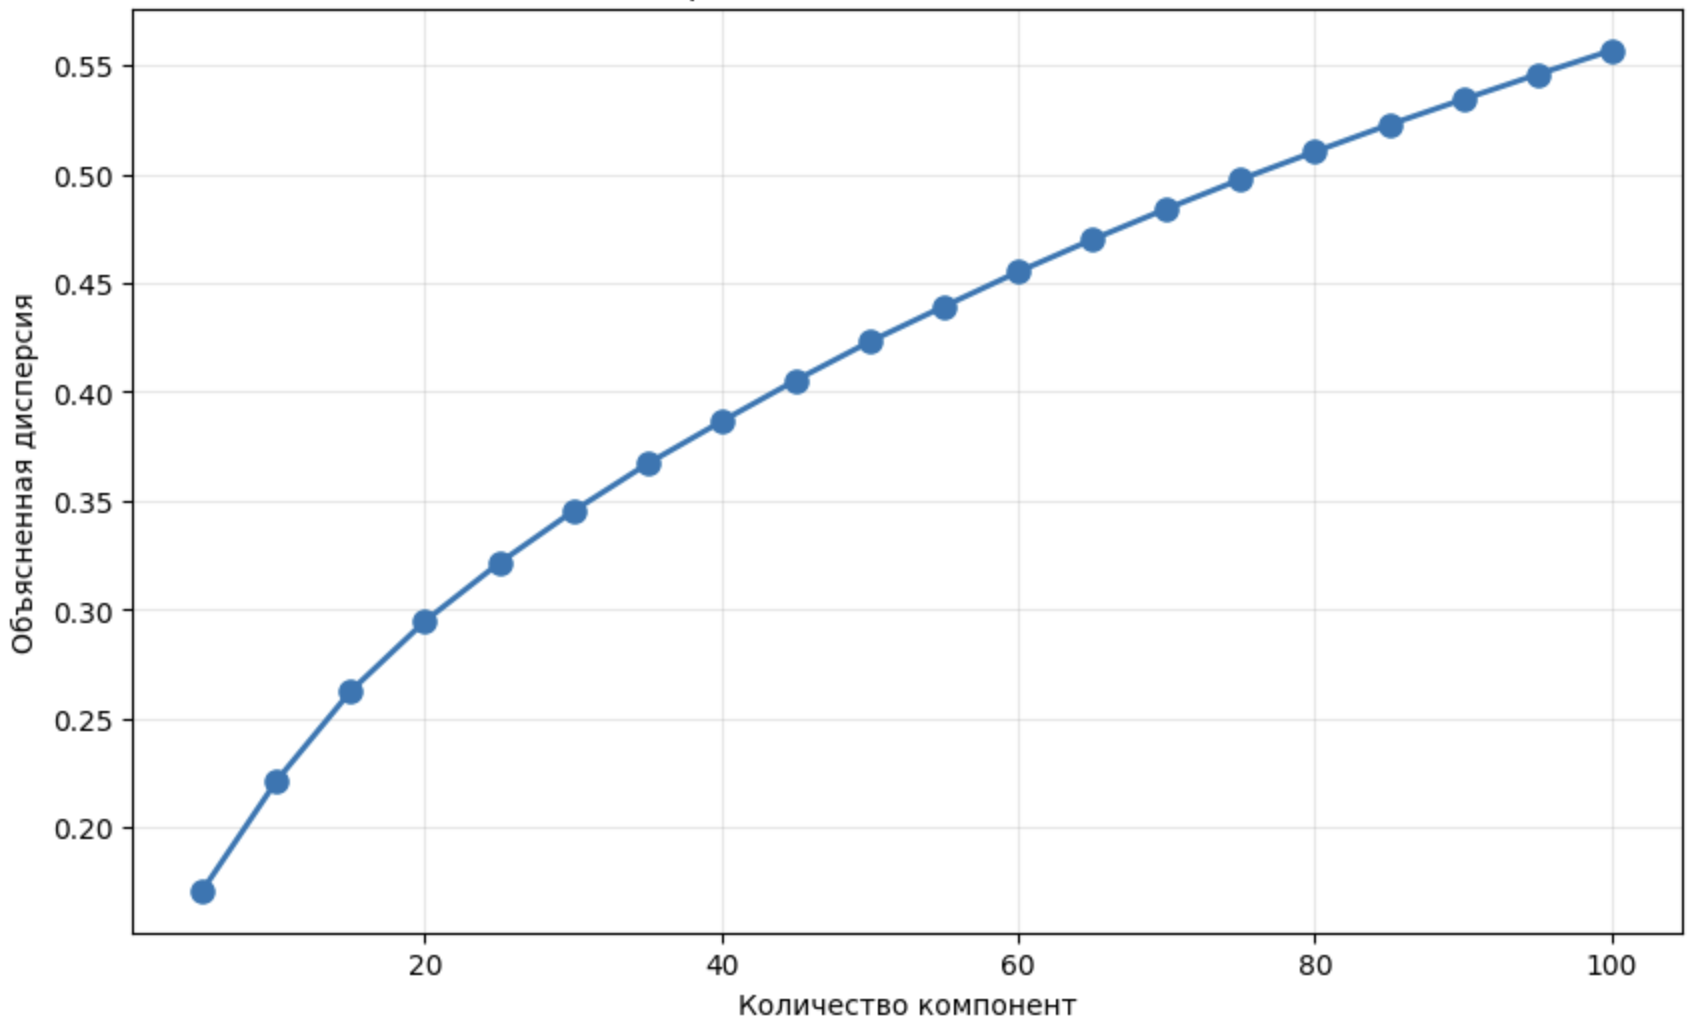
\includegraphics[width=\textwidth]{images/2.png}
	\end{center}
	\caption{Зависимость значения объяснённой дисперсии от количества компонент SVD}
	\label{img:2}
\end{figure}

Для подбора оптимального количества скрытых факторов (компонент разложения SVD) было проведено обучение моделей для значений от 5 до 100 с шагом 5. Зависимость значений объяснённой дисперсии и ошибки RMSE от количества компонент SVD приведено на рисунках \ref{img:2} и \ref{img:3}.

\begin{figure}
	\begin{center}
		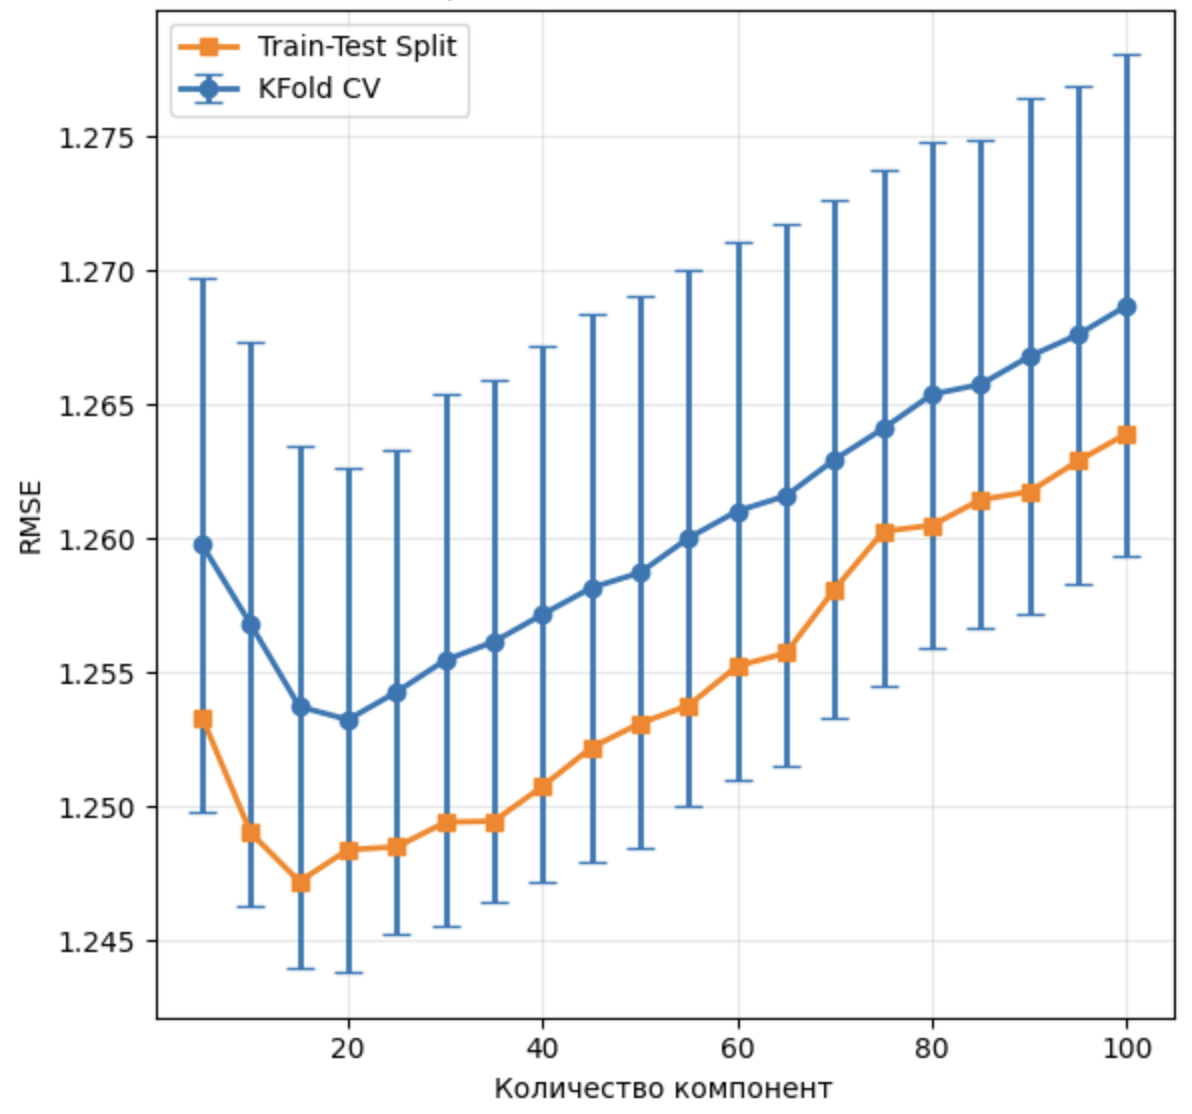
\includegraphics[width=\textwidth]{images/3.png}
	\end{center}
	\caption{Зависимость значения ошибки RMSE от количества компонент SVD}
	\label{img:3}
\end{figure}

Минимальное значение ошибки RMSE было достигнуто пр использовании 15 скрытых факторов. Примеры рекомендаций обученной системы приведены в листинге \ref{lst:1}.

\begin{lstlisting}[label=lst:1,caption=Примеры рекомендаций для пользователей]
	@Пользователь@: 65962952
	@Оценённые игры@:
	1. Aliens vs. Predator

	@Рекомендуемые игры@:
	1. Call of Duty Modern Warfare 2 - Multiplayer (@оценка@: 0.0016)
	2. Left 4 Dead 2 (@оценка@: 0.0016)
	3. Call of Duty Black Ops (@оценка@: 0.0012)
	4. Call of Duty Modern Warfare 2 (@оценка@: 0.0012)
	5. Call of Duty Modern Warfare 3 - Multiplayer (@оценка@: 0.0010)
	--------------------------------------------------
	@Пользователь@: 10253354
	@Оценённые игры@:
	1. Fallout 4
	2. Spore
	3. Fallout New Vegas
	4. Left 4 Dead 2
	5. Tomb Raider
	... @и ещё 127 игр@
	
	 @Рекомендуемые игры@:
	1. Napoleon Total War (@оценка@: 0.8531)
	2. PAYDAY 2 (@оценка@: 0.7533)
	3. Just Cause 2 (@оценка@: 0.6823)
	4. Metro 2033 (@оценка@: 0.6795)
	5. War Thunder (@оценка@: 0.6570)
\end{lstlisting}

\clearpage
